\section{Temporal Analysis}

TODO: zusammen fassen das alles gleich ist!\\
nur degree und closeness etwas mehr beschreiben.\\
The edge weight distribution is the same for all three snapshots (figure~\ref{fig:statEdgeWeightDist}).
The same is true for the correlation between the age of bees and the frequency this bee was detected (figure).


same degree distribution, can be seen in figure X\\
same strength distribution and same local clustering coefficient distribution (figure are in appendix)\\
figure degee distribution\\
maybe: relation to age and detection frequency also in appendix\\



same centrality distribution betweenness is in appendix\\
figure for closeness distribution\\
maybe relation to age and detection frequency also in appendix\\



%%%%%%%%%%%%%%%%%%%%%%%%%%%%%%%%%%%%%%%%%%%%%%%%%%%%%%%%%%%%%%%%%%%%%%%%%%%%%%%
\subsection{Stable Communities}
%%%%%%%%%%%%%%%%%%%%%%%%%%%%%%%%%%%%%%%%%%%%%%%%%%%%%%%%%%%%%%%%%%%%%%%%%%%%%%%
Table~\ref{tab:communities} lists the exact number of bees per community for each algorithm and snapshot.
For each snapshot, the leading eigenvector detected two communities with about the same number of bees.
The first communities CY(1,2,3) contain the queen and on average younger bees than the second communities CO(1,2,3).\\
In comparison, walktrap identified three communities, but two for the first snapshot.
Again the first communities CY(1,2,3) consist of the queen and on average younger bees than the second CM(2,3) and third communities CO(1,2,3).
The bees in CM2 and CM3 are on average younger than the bees in CO2 and CO3.
Figure~\ref{fig:ageDistribution} depicts the age distribution for each community and snapshot.

A two-sample Kolmogorov–Smirnov test showed that the age distributions are significantly different ($p< 0.001$) for both algorithms. However, the $p$-values for the walktrap communities CM2, CO2, and CM3, CO3 are lower.

CY(1,2,3) are located in the center of the comb, CO(1,2,3) closer to the hive access and CM(2,3) are situated in between. This spatial segregation of communities is similar in all three snapshots. For further reference see heat maps in~\ref{fig:communitiesPerNetworkWT} and~\ref{fig:communitiesPerNetworkLE}.


Functional groups of honey bees seem to differ in their respective age and occupy different areas of the comb.


\begin{table}
\centering
\caption[Overview about communities]{\textbf{Overview about communities per network} Communities marked with * contain the queen. Age and standard deviation (SD) are measured in days. For each network the queen and bees with a negative agre are excluded: network 1 - 12 bees, network 2 - 119 bees, network 3 - 10 bees.}
\label{tab:communities}
\vspace*{5mm}
\begin{tabular}{lcrrrrr}
	\toprule
	{}  & ID & Members & Proportion & Age & SD\\
	\midrule
	\rowcolor{Gray}
	Leading eigenvector &&&&&\\
	\midrule 
	\quad Network 1  & CY1 & $*430$  & 47.25\% & $17.12$ & $\pm10.97$ \\
	                 & CO1 & $480$   & 52.75\% & $27.24$ & $\pm10.96$ \\
	\midrule   							
	\quad Network 2  & CY2 & $*392$  & 45.63\% & $20.24$ & $\pm12.01$ \\
	                 & CO2 & $467$   & 54.37\% & $28.10$ & $\pm10.88$ \\
	\midrule  
	\quad Network 3  & CY3 & $*381$  & 41.78\% & $13.15$ & $\pm13.50$ \\
	                 & CO3 & $531$   & 58.22\% & $28.70$ & $\pm11.67$ \\
    \midrule
    \rowcolor{Gray}
    Walktrap &&&&&\\
    \midrule 
	\quad Network 1 & CY1 & $*427$ & 46.92\% & $17.07$ & $\pm10.92$\\
	                & CO1 & $482$  & 52.97\% & $27.23$ & $\pm11.00$\\
	\midrule
	\quad Network 2 & CY2 & $*263$ & 30.62\% & $18.23$ & $\pm11.46$\\
				    & CM2 & $305$  & 35.51\% & $25.20$ & $\pm11.47$\\
				    & CO2 & $291$  & 33.88\% & $29.47$ & $\pm10.06$\\            
	\midrule
	\quad Network 3 & CY3 & $*229$  & 25.11\% & $6.55$  & $\pm10.36$\\
					& CM3 & $298$  & 32.68\% & $25.08$ & $\pm11.97$\\
					& CO3 & $385$  & 42.21\% & $29.29$ & $\pm11.44$\\
	\bottomrule
\end{tabular}
\end{table}
\begin{table}
\centering
\caption[Kolmogorov-Smirnov test]{\textbf{Kolmogorov-Smirnov test} $p$-values for leading eigenvector (LE) and walktrap (WT) for each network and its communities.}
\label{tab:pvalues2}
\vspace*{5mm}
\begin{tabular}{lcrrrrr}
	\toprule

	\rowcolor{Gray}
	 & & LE p-value & WT p-value\\
	\midrule 
	\quad Network 1     & CY1, CO1 & 2.18e-33 & 1.52e-32 \\
	\midrule   							
	\quad Network 2     & CY2, CO2 & 2.99e-20 & 2.3e-32 \\
					    & CY2, CM2 &          & 4.72e-10\\
					    & CM2, CO2 &          & 1.00e-04\\
	\midrule  
	\quad Network 3     & CY3, CO3 & 5.10e-66 & 5.51e-67\\
					    & CY3, CM3 &          & 1.10e-95\\
						& CM3, CO3 &          & 1.98e-05\\ 
	\bottomrule
\end{tabular}
\end{table}


%%%%%%%%%%%%%%%%%%%%%%%%%%%%%%%%%%%%%%%%%%%%%%%%%%%%%%%%%%%%%%%%%%%%%%%%%%%%%%%
\subsection{Dynamic of Community Members}
%%%%%%%%%%%%%%%%%%%%%%%%%%%%%%%%%%%%%%%%%%%%%%%%%%%%%%%%%%%%%%%%%%%%%%%%%%%%%%%
Figure~\ref{fig:membersLE} (leading eigenvector) and figure~\ref{fig:membersWT} (walktrap) show the flow of  community members between consecutive snapshots.
For leading eigenvector communities, the majority of the bees stay in their age group, and a small fraction of bees switches to older communities.
Only a few bees change to younger communities.
The new middle-aged communities CM2 and CM3, detected by walktrap, consist partly of young (CY1) and old (CO1) bees. The switching behavior of individuals between communities is similar to leading eigenvector.

Individual bees change communities as they age.

\begin{figure}[htb]
	\centering
	\begin{subfigure}[b]{1.0\textwidth}
	\centering
	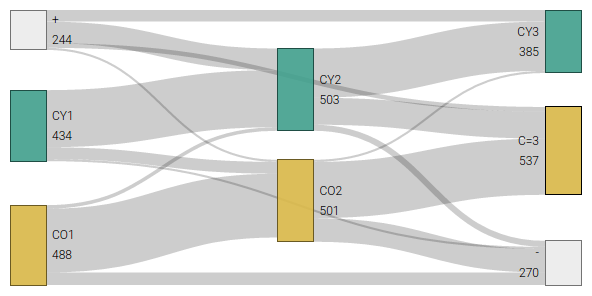
\includegraphics[width=.8\textwidth]{Figures/le_matching}
	\caption[Leading eigenvector communities]{Leading eigenvector communities}
	\label{fig:membersLE}
	\vspace*{5mm}
	\end{subfigure} 
	\begin{subfigure}[b]{1.0\textwidth}
	\centering
	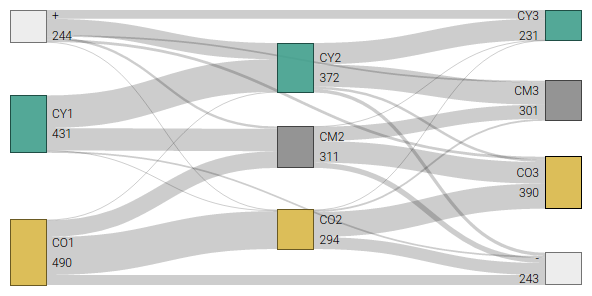
\includegraphics[width=.8\textwidth]{Figures/wt_matching}
	\caption[Walktrap communities]{Walktrap communities}
	\label{fig:membersWT}
	\vspace*{5mm}
	\end{subfigure}
	\caption[Dynamic community members]{\textbf{Dynamic community members} 
	Each column represents a time step, the colored rectangles represent the communities for each time step, and the height of the rectangles corresponds to the number of its community members, as referenced by the number. \emph{Green} indicates the community containing young bees and the queen, \emph{gray} represents the community containing middle-aged bees (only for walktrap), and \emph{orange} the community containing old bees. This figure shows that the major part of the members eighter stay in the same aged community or switch to an older group.}
	\label{fig:members}
\end{figure}
